% Generated by paper4/manuscript/build.py from paper4/paper/section_E10geo.md (d8c358fe143a1f8f): edit the Markdown, not this file.
\subsection{Where: placement and proximity (E10-geo)}
The label signal lies within about 250 m of an instrumented segment, so placement can matter only through how many uncovered segments it puts within that radius. E10-geo measures this for three rules at the same number of sensors, with 20 draws each: \textbf{blocks} (the whole-cell corridors of E9), \textbf{uniform} (segments drawn at random) and \textbf{density-stratified} (equal numbers from five strata of local density, which oversamples sparse areas).

\begin{figure*}[!t]
\centering
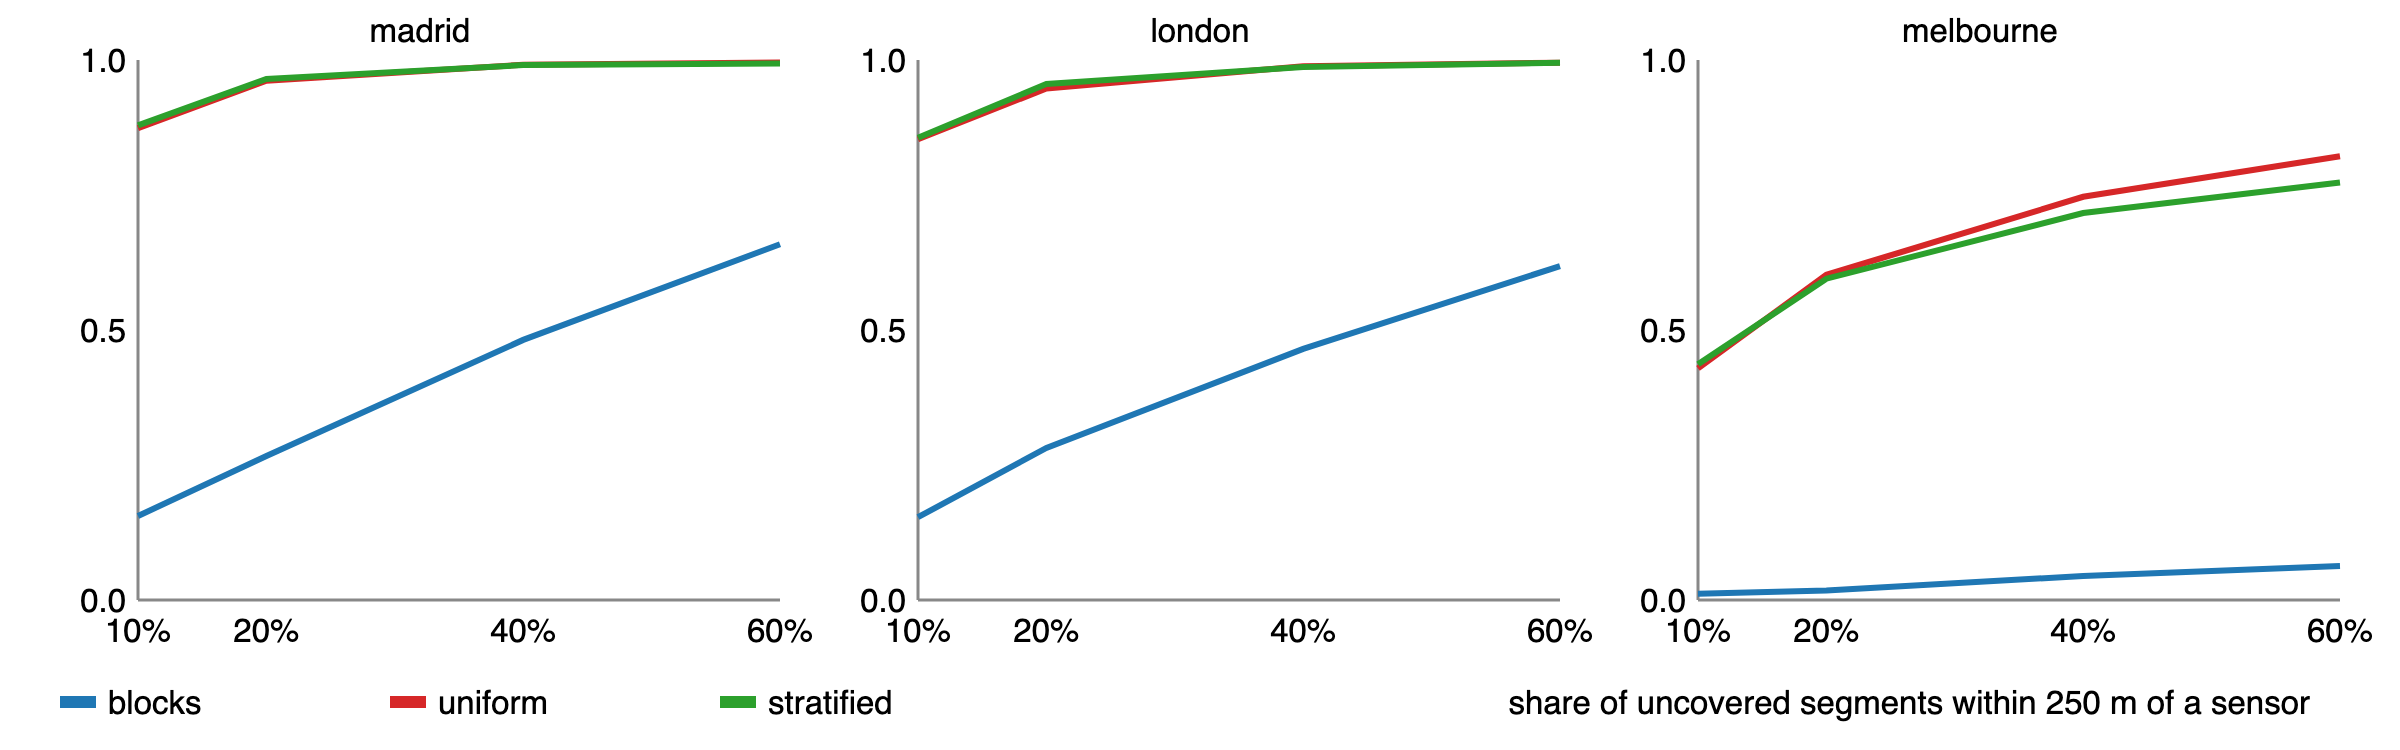
\includegraphics[width=\textwidth]{figures/e10geo_curva.png}
\caption{Share of uncovered segments with an instrumented segment within 250 m, against coverage. One panel per city; one line per rule (blocks, uniform, density-stratified); mean over 20 draws. Frozen figure \texttt{e10geo\_curva.svg} (a4edbde30583b455).}
\label{fig:e10geo}
\end{figure*}

\begin{table*}[!t]
\centering\footnotesize
\renewcommand{\arraystretch}{1.15}
\caption{Where: placement and proximity (E10-geo). Share of uncovered segments within 250 m of a sensor: mean over 20 draws, with the 2.5–97.5\% range. 10\% and 60\% shown; all levels in the frozen record and in Fig. 1.}
\begin{tabularx}{\textwidth}{>{\raggedright\arraybackslash\hsize=0.671\hsize}X>{\raggedright\arraybackslash\hsize=0.305\hsize}X>{\raggedright\arraybackslash\hsize=1.341\hsize}X>{\raggedright\arraybackslash\hsize=1.341\hsize}X>{\raggedright\arraybackslash\hsize=1.341\hsize}X}
\toprule
\textbf{City} & \textbf{\emph{f}} & \textbf{Blocks} & \textbf{Uniform} & \textbf{Density-stratified} \\
\midrule
Madrid & 10\% & 0.155 [0.078; 0.217] & 0.874 [0.785; 0.937] & 0.879 [0.810; 0.939] \\
Madrid & 60\% & 0.659 [0.453; 0.832] & 0.996 [0.991; 1.000] & 0.993 [0.983; 1.000] \\
London & 10\% & 0.153 [0.056; 0.225] & 0.853 [0.779; 0.929] & 0.856 [0.794; 0.929] \\
London & 60\% & 0.619 [0.493; 0.740] & 0.995 [0.989; 1.000] & 0.995 [0.986; 1.000] \\
Melbourne & 10\% & 0.012 [0.002; 0.023] & 0.429 [0.343; 0.494] & 0.436 [0.375; 0.515] \\
Melbourne & 60\% & 0.063 [0.027; 0.104] & 0.821 [0.757; 0.862] & 0.773 [0.739; 0.804] \\
\bottomrule
\end{tabularx}
\end{table*}

\textbf{Placement changes proximity by a large factor.} In Madrid and London, uniform placement at 10\% coverage puts 85–87\% of the uncovered segments within 250 m of a sensor, more than block placement reaches at 60\% (62–66\%); the median distance to the nearest sensor falls from 775–786 m with blocks to 94–109 m. From 20\% coverage, uniform placement brings at least 94.7\% within the radius. In Melbourne block placement leaves almost every uncovered segment beyond 250 m, and uniform placement brings 43–82\% within it. Oversampling sparse areas buys nothing: the density-stratified rule matches the uniform one within 0.01 in Madrid and London.

\textbf{What this proximity is worth.} Within 250 m, the calibrated neighbour stays 1–3 points behind G0 in Madrid and London, and net of the calendar it is worth nothing (§III-C). Placement therefore decides where the network measures, which segments carry a sensor and which lie next to one, but not how well the others are forecast.

\begin{quote}
\textbf{At the same number of sensors, the placement rule decides whether one uncovered segment in seven or six in seven lies within 250 m of a sensor in Madrid and London; that proximity buys no forecast.}
\end{quote}

